% -*- mode: fundamental -*-

% ****************************************************************

\chapter{BSV: Struct types, tuples, and\\
RISC-V: Memory requests and responses}

\markboth{Ch \arabic{chapter}: BSV structs; RISC-V mem reqs and rsps}{\copyrightnotice}

\setcounter{page}{1}
% \renewcommand{\thepage}{\arabic{page}}
\renewcommand{\thepage}{\arabic{chapter}-\arabic{page}}

\label{ch_Structs_Mem_Reqs_Rsps}

% ****************************************************************

\section{RISC-V: structs communicated between steps}

\index{BSV!struct!hetoregeneous collection of values}
\index{BSV!field!of a {\tt struct}}
\index{BSV!member!of a {\tt struct}}

Various kinds of information need to be communicated between the steps
of Figure~\ref{Fig_Instr_Exec}---program counter values, instructions,
values read from registers, values to be written back to registers,
and so on.  \verb|struct| data types (short for ``structures'') are
suitable for bundling together heterogeneous collections of values.
(This is the same concept in C and SystemVerilog; it is also called a
``record'' in some programming languages.)  Each component of a struct
is called a ``field'' or a ``member'' of the struct.
\begin{figure}[htbp]
  \centerline{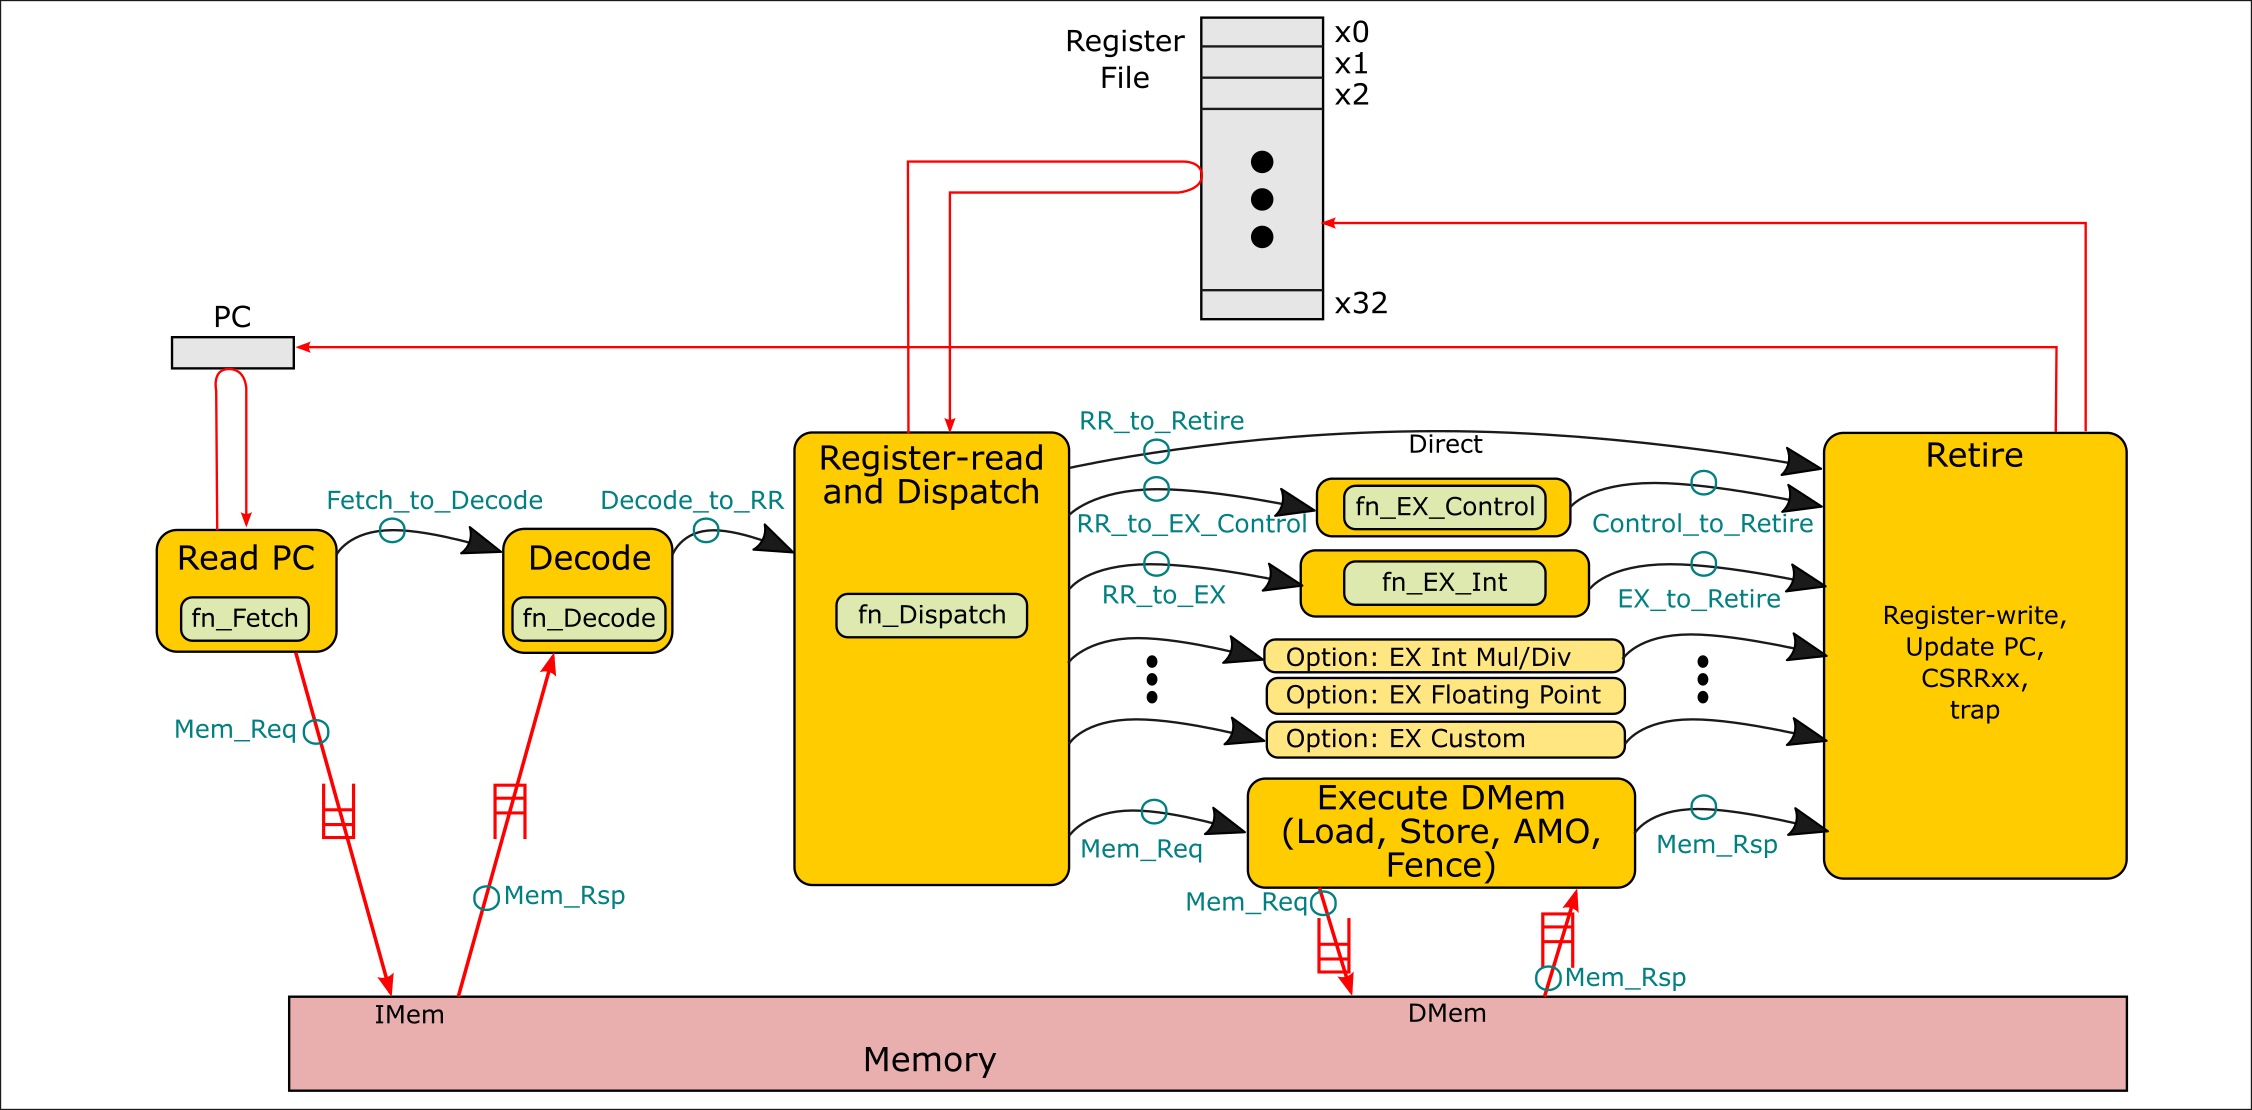
\includegraphics[width=6in,angle=0]{Figures/Fig_Instr_Exec_w_structs}}
  \caption{\label{Fig_Simple_Instr_Exec_w_structs}
           Simple interpretation of RISC-V instructions
	   (Fig.~\ref{Fig_Instr_Exec} with arrows annotated with {\tt struct} types)}
\end{figure}
Figure~\ref{Fig_Simple_Instr_Exec_w_structs} annotates
Figure~\ref{Fig_Instr_Exec} with struct types communicated on each of
the black arrows between steps, and each of the red arrows to and from
memory.  In this and the next few chapters we will flesh out the
details of all these struct types.  We will use exactly the same
struct types for Fife and Drum, {\ie} whether the implementation is
pipelined or not.  All these \verb|struct|
declarations can be found in the file: \verb|src_Common/Inter_Stage.bsv|.

% ****************************************************************

\section{BSV: {\tt struct} types}

\label{BSV_struct_types}

Consider the black arrow from the Decode step to the
Register-read-and-Dispatch step of
Figure~\ref{Fig_Simple_Instr_Exec_w_structs}.
We want to communicate several values, including:

\begin{itemize}

\item The current PC.  This will be needed by BRANCH, JAL, JALR and
  AUIPC instructions to compute addresses that are offset from the
  current PC.  It will be needed for any traps (exceptions) that may
  occur, which save PC for the trap-handler.

\item An \verb|exception| flag, indicating:

  \begin{tightlist}

    \item whether an error was encountered in the Fetch-to-Memory-to-Decode path, or

    \item whether the Decode step's analysis indicates that the
        instruction is not legal (unrecognized 32-bit code).

  \end{tightlist}

  When the exception flag is true, a \verb|cause| field provides more detail.

\item If there is no exception (no Fetch memory error; instruction is
legal), other fields provide more analytical detail for subsequent steps:

  \begin{tightlist}

    \item The ``fall-through'' PC, {\ie} the address of the next
      instruction following this one in memory.  For RV32I and RV64I,
      this will always be PC+4, since all instructions are 4-bytes
      long.\footnote{If we implement the ``C'' RISC-V ISA extension
      (compressed instructions), the correct fall-through PC may be
      PC+2.}  For most instructions, the fall-through PC is indeed the
      unique next PC.  For conditional BRANCH instructions, this is
      the next PC if the BRANCH is not taken.  For JAL and JALR
      instructions (unconditional jumps), this is the ``return
      address'' saved by the instruction in a register.

    \item The instruction itself.  This will be needed for opcode
      details, the rs1, rs2 and rd register indexes, immediate values,
      {\etc}
  \end{tightlist}

  The next several fields are derived by analyzing the instruction.
  They could be re-derived wherever needed by re-analyzing the
  instruction, but we perform that work just once in the Decode step
  and communicate the results.

  \begin{tightlist}

    \item The \verb|OpClass|.  This indicates to which next-step in
      Figure~\ref{Fig_Simple_Instr_Exec_w_structs} we dispatch for
      subsequent actions.

    \item Whether the instruction reads rs1 and/or rs2 register
      values.  This will be needed to control reading from the
      register file.

    \item Whether the instruction writes an rd register value.  This
      will be needed to control writing to the register file.

    \item The ``immediate'' value in the instruction. Refer to the top
        of each page of ``Table 24.2 Instruction listing for RISC-V''
        in the Unprivileged Spec~\cite{RISCV_Unpriv_2019_12_13}, which
        shows that the I-, S-, B-, U- and J-type instructions have
        immediate values of different sizes and encode them in
        different ways (``bit-swizzled'').  We untangle these once in
        the Decode stage, and pass on the clarified results in the
        \verb|imm| field.
  \end{tightlist}

\end{itemize}

This heterogeneous collection of values is most conveniently expressed
as a \verb|struct| type:

\label{Sec_struct_D_to_RR}

\index{BSV!struct@{\tt struct}!type declaration}

\input{Code_Extracts/Decode_to_RR.tex}

\index{BSV!deriving!Bits}

Because we said ``\verb|deriving(Bits)|'', the \emph{bsc} compiler
will automatically work out a representation for \verb|Decode_to_RR|
values in bits, using the straightforward method of simply
concatenating the bit-vectors of each field into a bit-vector for the
whole struct.  The total bit-size of a \verb|Decode_to_RR| struct
value is simply the sum of the individual bit-sizes of the fields.  If
we had not said ``\verb|deriving(Bits)|'', we could explicitly provide
some other custom representation in bits.\footnote{ In C/C++,
compilers will often ``pad'' out fields (insert unused bits between
fields) to be aligned on byte and word boundaries, for more efficient
access in byte-structured memories; thus, a struct's size in C/C++ may
be larger than the sum of the field sizes, and may even vary depending
on the compiler's target architecture.  In hardware design, these
values may reside in wires, registers, FIFOs, etc which have no
``byte-structured'' bias, and so we do not play any such ``padding''
games.}

\index{BSV!packing of struct fields and vector elements}
\index{BSV!structs!packing of fields}
\index{BSV!vectors!packing of fields}

% ----------------
\vspace{2ex}

NOTE:
\fbox{\small
\begin{minipage}{5in}

SystemVerilog makes a distiction beteen ``packed'' and ``unpacked'' values.

\vspace{2ex}

In BSV all struct and vector values are packed (no padding between
fields/elements) unless the user has explicitly over-ridden the
``deriving (Bits)'' directive with their own bit-representation
function.

\end{minipage}}
% ----------------

% ----------------
\vspace{2ex}

CAVEAT:
\fbox{\small
\begin{minipage}{5in}

Unfortunately Verilog, the target language for the \emph{bsc}
compiler, does not have any concept of structs.  When debugging
Verilog code that has been produced by \emph{bsc} from BSV source
code, a struct will appear as a flat bit-vector that aggregates all
the fields.

\end{minipage}}
% ----------------

\index{BSV!deriving!Fshow}

Because we said ``\verb|deriving(FShow)|'', the \emph{bsc} compiler
will automatically define an ``\verb|fshow()|'' function for this
type: if we print \verb|fshow(|\emph{v}\verb|)|, it will print
something like this:

{\small
\begin{Verbatim}[frame=single, numbers=left]
Decode_to_RR {pc=..., exception = ..., instr=..., ... }
\end{Verbatim}
}

% ================================================================

\subsection{Creating struct values}

\index{BSV!struct!entire struct values}

We can create a new value of type \verb|D_to_RR| with syntax like
this:

{\small
\begin{Verbatim}[frame=single, numbers=left]
   Decode_to_RR x = Decode_to_RR {pc:           ... value of field ... ,
                                  exception:    ... value of field ... ,
                                  cause:        ... value of field ... ,
                                  fallthru_pc:  ... value of field ... ,
                                  instr:        ... value of field ... ,
                                  ...};
\end{Verbatim}
}

The right-hand side is sometimes called a ``struct expression'', {\ie}
it is an expression which, when evaluated, produces a struct value.

The repetition of \verb|Decode_to_RR| above seems verbose; the
left-hand side instance is the type, and the right-hand side instance
is the ``struct constructor'' (think of it as a function that takes
the field values as arguments and returns a struct value). The
\emph{bsc} compiler's type-analysis is able to infer the type from the
right-hand side, so we can just use the keyword ``\verb|let|'':

\index{BSV!let@{\tt let}!binding an identifier with implicit type declaration}
\index{let@{\tt let}: BSV, binding an identifier with implicit type declaration}

{\small
\begin{Verbatim}[frame=single, numbers=left]
   let x = Decode_to_RR {pc:           ... value of field ... ,
                         exception:    ... value of field ... ,
                         cause:        ... value of field ... ,
                         fallthru_pc:  ... value of field ... ,
                         instr:        ... value of field ... ,
                         ...};
\end{Verbatim}
}

The order in which the field values are given does not matter; the
\emph{bsc} compiler will put the fields into the correct offsets in
the struct value.

% ================================================================

\subsection{Don't-care values} 

\label{Sec_Dont_Care_Values}

\index{BSV!Don't care literal value ``?''}
\index{BSV!?@{\tt ?} (don't care literal value)}

Not all field values need be given in a struct expression.  The
\emph{bsc} compiler will issue a warning for each unspecified field,
and insert an ``unspecified'' (and unpredictable) value there.  You
can indicate that a field is intentionally left unspecified (and
suppress the compiler warning) using ``\verb|?|'', BSV's notation for
a ``don't care'' value:

\index{BSV!{\tt ?}, the don't care value}
\index{BSV!AAAA\_AAAA, the default don't care value}

{\small
\begin{Verbatim}[frame=single, numbers=left]
      let x = Decode_to_RR {pc:           ... ,
                           exception:    False,
                           cause:        ?,
                           fallthru_pc:  ... ,
                           instr:        ... ,
                           ...};
\end{Verbatim}
}

In the above example, the exception \verb|cause| field is meaningless
when the \verb|exception| field is false, and we indicate this
explicitly with ``\verb|?|''.

``Don't care'' values are useful for several reasons.  First, this
conveys to the human reader that the value in this field is
irrelevant.

Second, it can result in more efficient circuitry.  If we had said
``0'', for example, the \emph{bsc} compiler has to create circuitry
ensuring that field's value is 0. By saying ``\verb|?|'', the
\emph{bsc} compiler is allowed to omit all that circuitry.

Third, in places where it does not result in additional hardware, the
\emph{bsc} compiler usually injects the specific value
\verb|'h_AAAA_AAAA| (of suitable bit-width).  While debugging,
observing such a value in some computation is often a clue that
something is wrong (it roughly plays the role of ``X'' values in
Verilog/SystemVerilog/VHDL).

% ----------------
\vspace{2ex}

\index{BSV!X values!Notation for unassigned values in Verilog (no such concept in BSV)}

NOTE:
\fbox{\small
\begin{minipage}{5in}

Verilog, SystemVerilog and VHDL have a concept of ``X'' values.  Each
bit of a register or wire carries an ``X'' value until it has been
assigned a specific binary value (0 or 1).  However, note that this is
\emph{only in simulation}, where the simulator can and does model
3-valued logic (0, 1 and X) for each bit, and is able to propagate X
values through operators, registers, {\etc} Hardware only implements
2-valued logic---every bit is either 0 or 1. Thus, this is an artefact
that is only useful during debugging in simulation and static
analysis.

\vspace{1ex}

BSV only has 2-valued logic; there is no concept of an ``X'' value.  A
BSV ``{\tt ?}'' expression has some specific, but potentially
unpredictable, binary value.

\end{minipage}}
% ----------------

% ================================================================

\subsection{Selecting struct fields}

\index{BSV!struct!field selection}

Struct fields can be selected using the usual ``dot'' notation common
to SystemVerilog and C/C++:

{\small
\begin{Verbatim}[frame=single, numbers=left]
   x.pc
   x.instr
\end{Verbatim}
}


% ================================================================

\subsection{Updating struct fields using assignment}

\index{BSV!struct!field assignment/update}

Struct fields can be updated with assignment using the usual ``dot''
notation common to SystemVerilog and C/C++:

{\small
\begin{Verbatim}[frame=single, numbers=left]
   x.pc    = ... new value ... ;
   x.instr = ... new value ... ;
\end{Verbatim}
}

% ****************************************************************

\section{BSV: Tuples and the {\tt match} statement}

\label{Sec_Tuples}

\index{BSV!Tuples}

Tuples are a built-in set of struct-like constructs in BSV that are
often convenient.  For example, when a function needs to return a pair
of values, instead of declaring a struct type with two fields for the
result, it is often more convenient to just use the built-in
\verb|Tuple2| type.  Example: (from the \verb|mkCSRs| module in file
\verb|src_Common/CSRs.bsv|):

{\small
\begin{Verbatim}[frame=single, numbers=left]
   function ActionValue #(Tuple2 #(Bool, Bit #(XLEN)))
            fav_csr_read (Bit #(12) csr_addr);
      ...
         let result = (exception, rd_val);
	 return result;
   endfunction
\end{Verbatim}
}

The function returns a pair of values which have types \verb|Bool| and
\verb|Bit#(XLEN)|, respectively.  The overall type of the result is
\verb|Tuple2 #(Bool, Bit #(XLEN))|.

The expression on the right-hand side of the \verb|let| statement
shows how one can construct a 2-tuple value: simply enclose the
components in parentheses and separate them with commas.

Unlike structs, there is no assignment statement to update a field of
a tuple, nor is there is any ``.field'' notation for component
selection.

To select an individual field of a tuple, one can use one of the
built-in selector functions:

{\small
\begin{Verbatim}[frame=single, numbers=left]
   let xy <- fav_csr_read (...);
   let exc = tpl_1 (xy);    // exc has type: Bool
   let v   = tpl_2 (xy);    // v   has type: Bit #(XLEN)
\end{Verbatim}
}

Alternatively, to access multiple fields of a tuple at once, one can
use a ``match'' statement. Example (from \verb|src_Drum/CPU_FSM.bsv|):

\index{BSV!Tuples|match@{\tt match} statement (pattern-matching_)}
\index{BSV!Pattern matching!match@{\tt match} statement for tuples}

{\small
\begin{Verbatim}[frame=single, numbers=left]
   match { .exc, .v } <- fav_csr_read (csr_addr);
\end{Verbatim}
}

The \verb|match| keyword is followed by a \emph{pattern} that should
match the tuple, {\ie} here it should be a list of two variable names
surrounded by braces with each variable preceded by a ``\verb|.|''.
The leading ``\verb|.|'' is important: ``\verb|x|'' would represent
the value of an existing variable to be matched with the corresponding
value in the tuple, whereas ``\verb|.x|'' \emph{introduces a new
variable} \verb|x| to be bound to the corresponding value in the
tuple; the latter is what we want.  We refer the reader to the BSV
Language Reference Guide~\cite{BSV_Lang_Ref_Guide} for many more
capabilities of pattern-matching, including fields to be ignored,
pattern-matching on structs and tagged unions, pattern-matching
\verb|case| expressions, and more.

BSV defines tuples of up to 8 components ({\tt Tuple\_3}, {\tt
Tuple\_4}, ...) but we recommend not using tuples when you have more
than, say, 2 or 3 components; define a struct instead, with readable
and meaningful field names.

% ****************************************************************

\section{RISC-V: Memory Requests and Responses; IMem and DMem}

\index{IMem| Instruction Memory}
\index{DMem| Data Memory}
\index{RISC-V!IMem (instruction memory)}
\index{RISC-V!DMem (data memory)}

In Figure~\ref{Fig_Simple_Instr_Exec_w_structs}, the \verb|Mem_Req|
and \verb|Mem_Rsp| structs are used in two places.  The Fetch step
issues a memory request, and the corresponding memory response is
received by the Decode step.  Similarly, the ``Execute Memory Ops''
steps issues a memory request and consumes a memory response.  We use
the shorthand term ``IMem'' for the first context (for Instruction
Memory) and ``DMem'' for the latter context (for Data Memory).

% ================================================================

\subsection{Separation of IMem and DMem (Harvard Architecture)}

\label{Sec_Harvard_architecture}

\index{Harvard architecture}
\index{Harvard architecture!Self-modifying code}

The separation of memory channels for instructions and data
(loads/stores) is quite standard in modern CPU architectures, and is
informally called a ``Harvard Architecture''.  The term refers to the
architecture of the Harvard Mark I computer, designed and built by
Harvard University and IBM in the 1940s (the term itself was coined
much later).  It sometimes refers just to separate, concurrent paths
to memory for instructions and data, and sometimes also to physically
separate memories for instructions and data (more discussion in
Wikipedia:~\url{https://en.wikipedia.org/wiki/Harvard_architecture}).

Modern software is typically not ``self-modifying'', {\ie}
instructions and data are placed in different areas of memory, and
load/store instructions never write into the instruction area, {\ie}
programs never over-write instructions in memory.  This allows
separate hardware for memory access for instructions {\vs} memory
access for data, which can run concurrently, {\ie} we may fetch an
instruction at the same time as we are accessing data memory for a
previous load/store instruction (we will see this in Fife).  We can
also tune and optimize each memory path separately for their different
dynamic behavioral patterns.  In some systems we can also
\emph{protect} the instruction memory area, {\ie} enforce in hardware
the policy of not over-writing instructions.

\index{JIT (Just-in-time compiling)}
\index{Just-in-time compiling (JIT)}

This view of strict separation of IMem and DMem has to be tempered
somewhat when considering languages like JavaScript, Python {\etc}
that employ so-called ``JIT'' compiling (``Just-In-Time'').  The
run-time systems of such languages generate instructions on-the-fly,
{\ie}, LOAD/STORE instructions produce \emph{data} through the DMem
channel that will (soon) be fetched as \emph{instructions}.  But even
in these systems, there is a strict protocol of \emph{phases}.  During
a code-generation phase, the data produced is considered as ordinary
data.  Then there is a deliberately executed phase-change, where the
virtual memory protections of the data-pages just written are changed
so that they are now viewed as read-only instruction pages, after
which these new instructions can be fetched.

% ================================================================

\subsection{Memory Requests}

\label{Sec_Mem_Req}

\index{Memory!Request}

A memory-request in RV32I is either a LOAD, a STORE or a FENCE.  We
could define an enum type for this:

{\small
\begin{Verbatim}[frame=single, numbers=left]
   typedef enum {MEM_REQ_LOAD,
                 MEM_REQ_STORE
		 MEM_REQ_FENCE} Mem_Req_Type
deriving (Eq, FShow, Bits);
\end{Verbatim}
}

which will use a 2-bit encoding (0 for LOAD, 1 for STORE, 2 for
FENCE).  However, we look to the future where we might extend Drum and
Fife to implement the ``A'' extension (for ``Atomic Memory
Operations'').  The RISC-V ISA Unprivileged Spec document, Chapter 8,
described additional memory operations LR (Load-Reserved), SC
(Store-Conditional), AMOSWAP, AMOADD, AMOXOR, AMOAND, AMOOR, AMOMIN,
AMOMAX, AMOMINU, and AMOMAXU, each of which comes in a 32-bit version
(in RV32 and RV64) and a 64-bit version (in RV64).  These operations
are coded with 5 bits in the instruction (\verb|instr[31:27]|).

Accordingly, we use a 5-bit encoding for LOAD, STORE and FENCE, using
5-bit codes that are not used in the A extension:

\input{Code_Extracts/funct5_MEMOPs.tex}

An IMem request is for one 32-bit instruction (four
bytes).\footnote{When implmenting the ``C'' RISC-V ISA extension
(compressed instructions), instructions can also be 16-bits (2 bytes).
When implementing more sophisticated Fetch units, we may actually
fetch much larger chunks, such as a full cache line.}  A DMem request
may be for one, two or four bytes.  We express these request-size
options using an enum type:

\input{Code_Extracts/Mem_Req_Size.tex}

A memory request bundles a request type, a size, and an address.  For
memory-writes, we also bundle the data to be stored.  We express this
bundle using a struct:

\input{Code_Extracts/Mem_Req.tex}

In \verb|Mem_Req_Size|, the option \verb|Mem_8B| is not possible in
RV32I.  Similarly, in \verb|Mem_Req| the \verb|addr| and \verb|data|
fields need only be 32-bits wide for RV32I.  However, we have declared
them as shown looking ahead into the future, where we may wish to
implement RV64I, or where we may wish to implement the ``D'' ISA
extension (double-precision floating point values, which are
represented in 64-bits).

For STORE requests of 1 and 2 bytes ({\ie} smaller than the \verb|data|
field) we assume the data is passed in the least-significant bytes of
the \verb|data| field.

This is the information sent to Memory from the Read-PC-and-Fetch step
and also from the Execute-Memory-Ops step in
Figure~\ref{Fig_Simple_Instr_Exec_w_structs}.

% ================================================================

\subsection{Address Alignment}

\index{Address alignment}
\index{Memory!Address alignment}

Although nowadays we think of all computer memories in units of 8-bit
bytes and being byte-addressed,\footnote{Some early computers, until
about the late 1970s, had other memory granularities---multiples of 6,
7, 9 bits, {\etc} Those were the days of bespoke memories for each
computer design.  Mass-production of memory chips resulted in
standardization to 8-bit bytes.} in practice in hardware, it is
usually simpler if memory-requests are \emph{aligned} to an address
according to the request size.  Specifically, the address for a 2-byte
request should be even, {\ie} the least significant bit of the
address, \verb|addr[0]|, should be zero.  The address for a 4-byte
request should have zero in the two least significant bits
(\verb|addr[1:0]|) and the address for an 8-byte request should have
zero in the three least significant bits (\verb|addr[2:0]|).

We can see why address-alignment is desirable.  Memory implementations
(chips) are usually architected to retrieve multiple bytes at a time
({\eg} 64 bytes) so that all those bytes can share addressing and
control circuitry.  With such an organization, a misaligned access
request may straddle the boundaries of such ``naturally sized'' units
and so may require two consecutive reads/writes.  Caches are usually
organized to hold multi-byte \emph{cache lines} ({\eg}, 32 bytes) in
order to share the addressing and miss-handling circuitry, and to move
data efficiently in and out of the cache.  Again, a misaligned access
request may straddle a cache-line boundary, and may require two
consecutive accesses, which may hit or miss independently.  Virtual
memory systems are usually organized in \emph{pages}, units of
typically 4K-8K bytes, in order to share virtual-memory handling
circuitry, and to move data efficiently between main memory and disks.
Again, a misaligned access may straddle a page boundary, and may
require two consecutive accesses, which may hit or page-fault
independently and differently.  In short, misaligned accesses add
significant complexity to memory-system hardware design.

We can organize our software so that misaligned accesses are
exceedingly rare.  Most software is produced by compilers, and the
compiler ensures that instructions and data are placed in memory at
aligned addresses, possibly by padding gaps between ``adjacent''
smaller-sized data (such as a pair of 1-byte-sized fields in a
struct).  This padding may waste a few bytes of memory, but pays back
in greater speed and reduced complexity.

Although misaligned accesses are rare, we cannot always guarantee
their absence in software, since software can calculate an arbitrary
address before performing a memory access.  It seems wasteful to have
to pay for extra hardware complexity (with attendant loss in overall
performance) for such rare cases.  In many computer systems,
therefore, these rare misaligned accesses are relegated to software
handling:

\begin{tightlist}

\item The memory system simply refuses to handle a misaligned access,
  and returns a ``misaligned'' error instead.

\item The CPU, receiving such an error response, undergoes a ``trap''
  which directs it to piece of software called an trap-handler (or
  exception handler).  The trap-handler (in software) performs the
  memory access in multiple smaller pieces (in the worst case, of size
  1 byte), each of which is aligned.  In other words, the trap-handler
  ``completes'' the original memory access before resuming the
  main-line code that attempted it.

\end{tightlist}

The RISC-V ISA specification does not forbid misaligned accesses nor
prescribe how they should be handled.  Some implementations will
handle it in hardware, and other implementations will return a
``misaligned'' error and rely on a trap handler to complete the
access.  Some implementations may only run software where it has been
proven to not generate misaligned memory requests, and therefore may
not even contain a trap-handler for misaligned accesses.

% ================================================================

\subsection{Memory Responses}

\label{Sec_Mem_Rsp}

\index{Memory!Response}

The response from memory for any request may be to report success, an
alignment error, or some other error.  Examples of ``other errors''
are:

\begin{itemize}

\item Absence of memory at the given address.  For example, although
  RV32I addresses are 32-bits, which can address 4GiB of memory, we
  may provision our system with something smaller, say 1 GiB.

\item An unsupported operation. {\Eg} an attempt to write into a
  read-only memory (ROM).

\item Corruption of data, due to electrical glitches, environmental
  electromagnetic pulses, {\etc}.  These errors are usually detected
  with some kind of error-detecting code, such as parity bits.

\end{itemize}

These different memory response-types can be encoded in an enum type:

\input{Code_Extracts/Mem_Rsp_Type.tex}

A memory-response contains the response-type. For a LOAD request with
an OK response, it also contains the data that was read from memory.
This can be expressed in a struct:

\input{Code_Extracts/Mem_Rsp.tex}

For LOAD requests of 1 and 2 bytes ({\ie} smaller than the \verb|data|
field) we assume the data is returned in the least-significant bytes
of the \verb|data| field.

% ****************************************************************
